\section{Allgemeine Vorgehensweise}
Im Folgenden wird die allgemeine Vorgehensweise beschrieben. Zur besseren Strukturierung, Dokumentierung und klaren Aufgabenverteilung, haben wir uns ein eigenes GitHub-Repository \footnote{https://github.com/HallerPatrick/AI-Birds-LeveGANerator} aufgesetzt, in welchem ebenfalls die Arbeitszeiten an den bestimmten Issues festgehalten wurden. Die wichtigsten Aufgaben werden in den nachfolgenden Unterkapiteln näher erläutert. [Graphen, allgemeine Struktur]
\begin{figure}
    \centering
    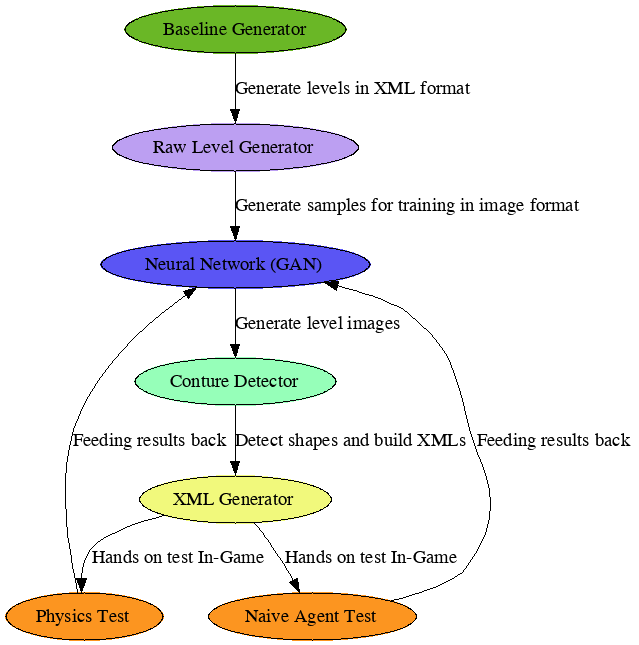
\includegraphics[height=12cm, width=10cm]{img/project_structure.png}
\end{figure}
\subsection{Erkennen der  Konturen von Zentroiden}
Um generell mit den generierten Bildern arbeiten zu können war es wichtig, diese erst durch die Erzeugung und Verstärkung der Konturen besser auf den Konturenerkenner abzustimmen. Nachfolgend möchten wir die Klasse \textit{conture\_detector.py} näher erläutern. \\
Zur allgemeinen Verarbeitung der Bilder bedarf es eines Imports der cv2-Klasse, welches zuvor installiert werden muss (unter OS X und Python3: \textit{"pip3 install opencv-python"}). In der Klasse wird nun das Bild ausgelesen und alle x- sowie y-Koordinaten in eine Liste \textit{*points} geschrieben. Das eingelesene Bild im HSV-Farbraum ("\textbf{h}ue": Farbwert, "\textbf{s}aturation": Farbsättigung, "\textbf{v}alue": Hell-/Dunkelwert)\footnote{https://de.wikipedia.org/wiki/HSV-Farbraum} wird in Graustufen umgewandelt, um Konturen innerhalb des Bildes zu ermöglichen (dieser Schritt kann allerdings auch übersprungen werden, da die Objekte verschiedene Farben aufweisen). \\ Zur Ermittlung der Zentroiden wird nun die Formel \[centrX = \sum XCoord / Length\] wobei folgende Zuweisungen gelten:
\begin{itemize}
	\item \(centrX\) entspricht den zu ermittelnden Zentroiden der X-Koordinaten (gilt analog für Y-Koordinaten mit \(centrY\))
	\item  \(\sum XCoord\) entspricht der Summe aller X-Koordinaten (gilt analog für Y-Koordinaten mit \(\sum YCoord\))
	\item  \(Length\) entspricht der Länge aller Punkte
\end{itemize}
\begin{figure}
	\centering
	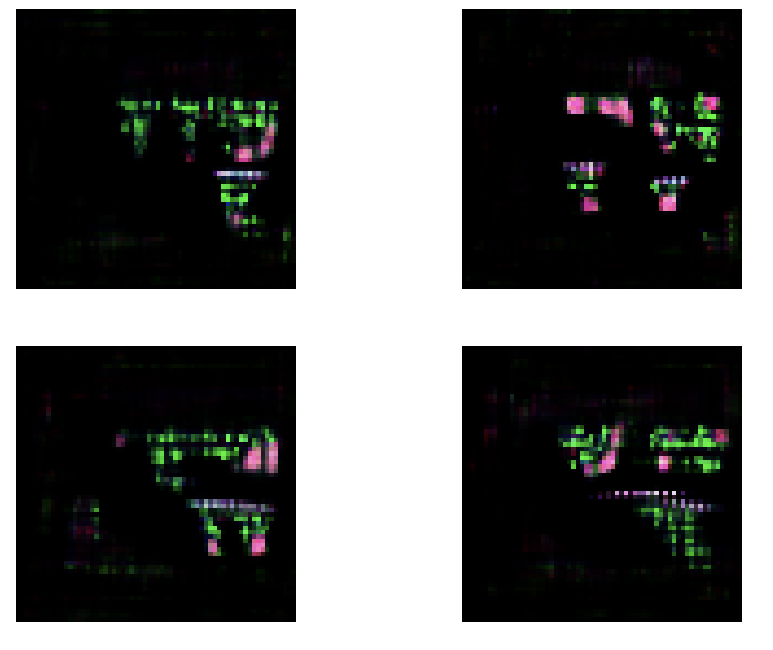
\includegraphics[height=10cm, width=10cm]{img/blurry_attempts.png}
	\caption{Verschwommene Konturen führen zu Problemen bei der Erkennung}
\end{figure}
\subsection{Automatisierung der Abläufe mithilfe von Powershell unter Windows}
Um zu vermeiden, dass alle Komponenten einzeln und umständlich gestartet werden müssen, haben wir es uns außerdem zur Aufgabe gemacht, ein Automatisierungsskript aufzusetzen, welcher diesen Schritt für uns übernimmt. Als Skriptsprache erschien uns PowerShell am sinnvollsten, da dieses ein fester Bestandteil von Windows 10 (dem gängigsten Betriebssystem) ist und aufgrund dessen keine extra Tools installiert und erläutert werden müssen. \\Das Skript startet zunächst ScienceBirds und skaliert diesen mithilfe von Window-Resizer (Tool zur nutzerbasierten Steuerung der Standardgröße eines Fensters, hier: ScienceBirds) auf einen bestimmten Wert, da der Agent sonst mit der Größe des ScienceBirds-Fensters nicht einverstanden ist. Im Anschluss wird der Agent und der Server automatisch in der Eingabeaufforderung gestartet. Wir konnten beobachten, dass durch den Startklick des Skripts alle benötigten Fenster ordnungsgemäß gestartet wurden und der Agent das Spiel wie erwartet, selbstständig gespielt hat.\\ In den folgenden Stichpunkten werden die einzelnen Fenster der Automatisierung näher erläutert (vgl. Abb.1).
\begin{itemize}
	\item[1)] Shell des Automators \\
	Aus diesem Fenster wird der Automator gestartet. Dazu wird zunächst überprüft, ob alle Umgebungsvariablen vorhanden und passend eingestellt sind, um volle Funktionalität gewährleisten zu können. Findet der Automator alle benötigten Tools, so wird der Nutzer gefragt, ob er diesen starten, den Vorgang abbrechen oder Umgebungsvariablen einstellen möchte.
	\item[2)] ScienceBirds-Fenster \\
	In diesem Fenster läuft das eigentliche Spiel. Da die Größe dieses Fensters für unseren Agenten nicht gepasst hat, musste ein Window-Resizer eingeschaltet werden, um ScienceBirds auf die benötigte Fenstergröße zu skalieren.
	\item[3)] AutoSizer-Fenster \\
	Hier befindet sich unser Window-Resizer. Dabei haben wir uns für den AutoSizer als Tool entschieden, da dieser wenig Speicherplatz einnimmt, kostenlos und ohne Bloatware zu installieren ist. Damit die Größe eines spezifischen Fensters auf einen immer gleichbleibenden Wert angepasst werden muss, haben wir im AutoSizer selbst einen Hotkey festgelegt, welcher beim Betätigen einer bestimmten Tastenkombination (hier: "\%9") die Größe von einem Fenster mit dem Namen "ScienceBirds" auf die benötigte Auflösung ändert. Diese Methode ist stark auf unser persönliches System abgestimmt, kann aber durch wenige Änderungen im Skriptcode auf die eigenen Parameter angepasst werden.
	\item[4)] Agent-Fenster \\ 
	Hieraus wird der Agent gestartet. Dazu wird zuerst der Agent gestartet und im Anschluss darauf der Server. Hier lässt sich beobachten, dass sich der Status von "Waiting" auf "Pending" ändert. Startet man nun den Agenten mit dem Klick auf "Start", so wechselt der Agent in den Status "Running".
	\item[5)] Server-Fenster
	Der Server muss gestartet werden um gewährleisten zu können, dass der Agent ordnungsgemäß läuft. Hier kann man die verschiedenen Aktionen beobachten, welche gerade stattgefunden haben (hier: "Go to Level Selection Page").
\end{itemize}
\begin{figure}
	\centering
	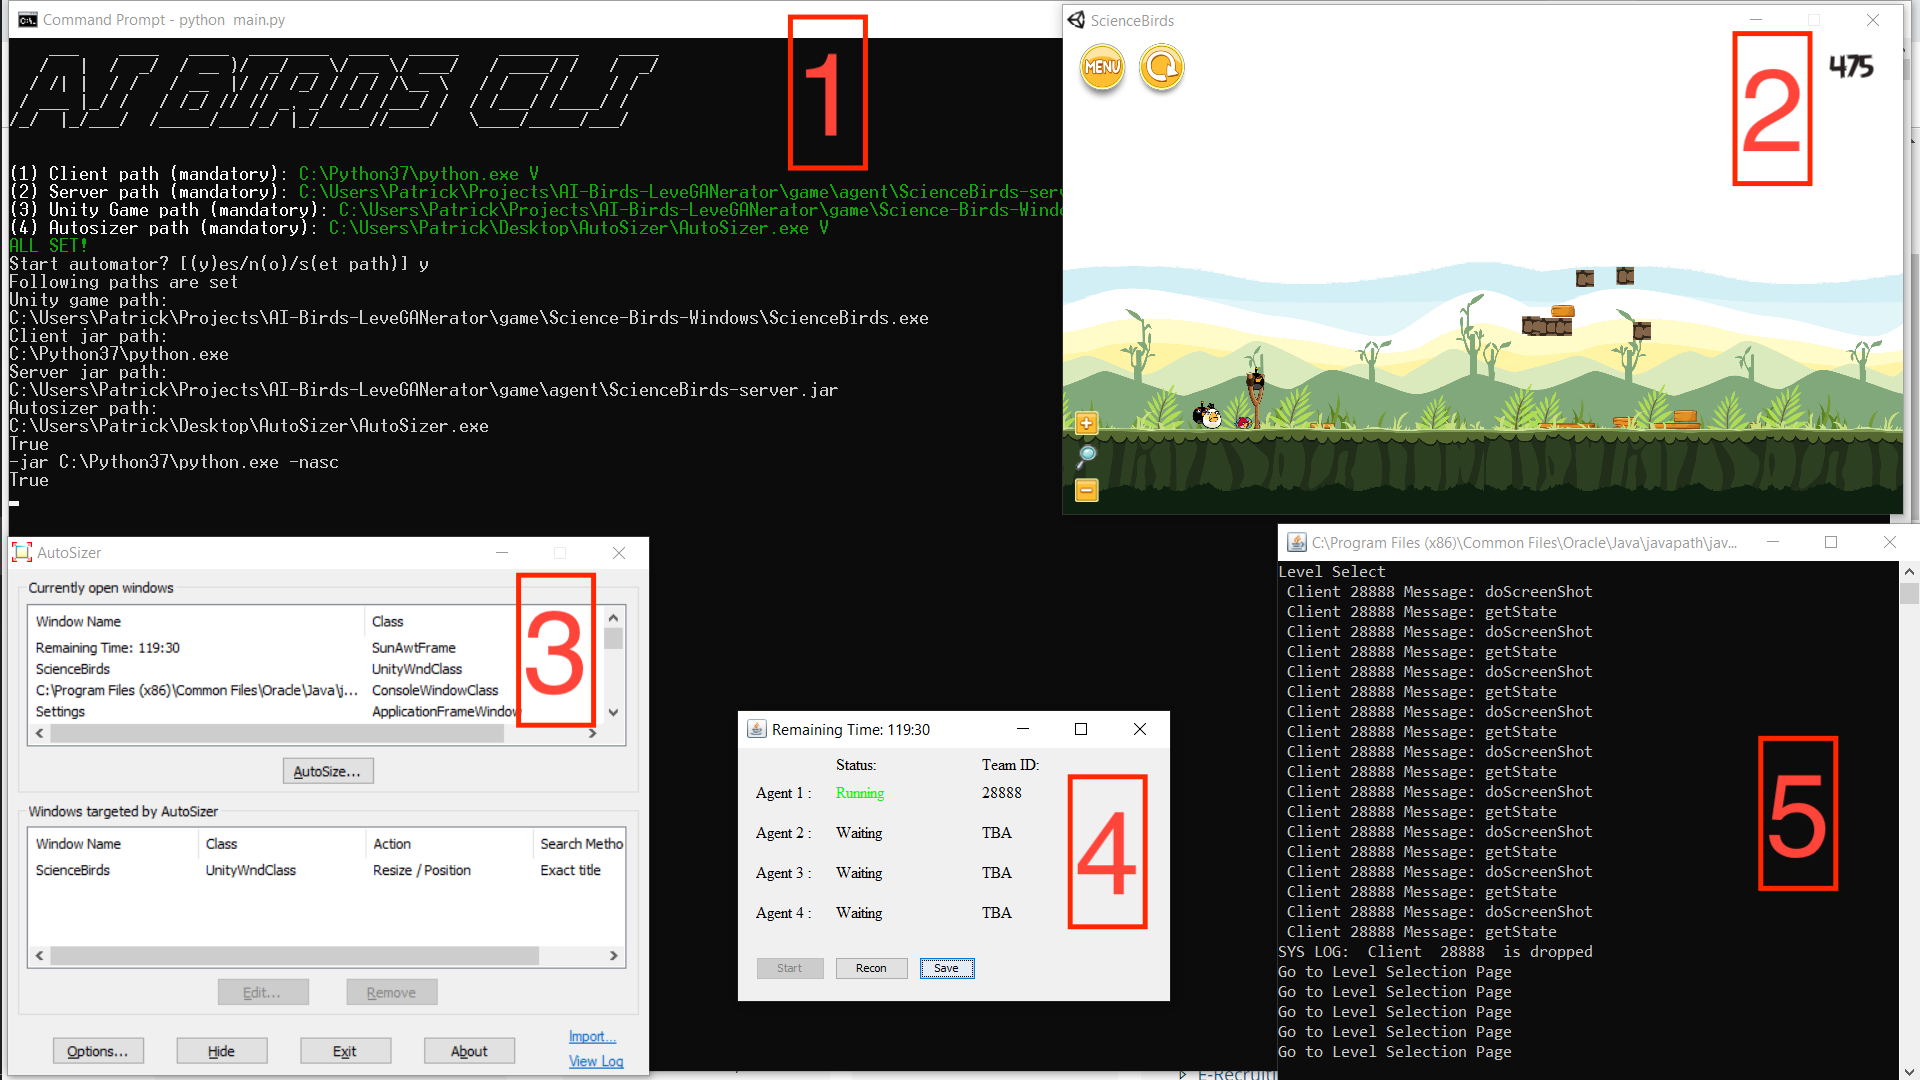
\includegraphics[height=9cm, width=16cm, clip]{img/automator_screen.png}
	\caption{Vorläufige GUI der Automatisierung}
\end{figure}
\subsection{Konvertierung von Pillow-Koordinaten in ein kartesisches XML-Koordinatensystem}
[Patrick]
\subsection{Verdeutlichen der Konturen der erzeugten RAW-Bilder zur besseren Erkennung vor Training}
Der Konturen-Erkenner hatte in unserem Durchlauf Probleme, die Umrisse der erzeugten Zentroide zu erkennen. Aufgrund dessen mussten wir die Konturen, welche erzeugt werden, vor dem Beginn des Trainings verstärken, damit diese eindeutig von unserem Erkenner gefasst werden können. 
\subsection{Aufsetzen eines Re-Evaluierungssystems}
[Patrick]